%        File: project.tex
%     Created: Mon Nov 07 08:00 PM 2011 M
% Last Change: Mon Nov 07 08:00 PM 2011 M
%
\documentclass[a4paper]{article}
\usepackage{amsmath}
\usepackage{minted}
\usepackage[pdftex]{graphicx}

\newcommand{\HRule}{\rule{\linewidth}{0.5mm}}
\begin{document}
\title{ % Upper part of the page
    \textsc{\LARGE CS 3100}\\[1.5cm]
    \textsc{\Large Final Project Report}\\[0.5cm]
    % Title
    \HRule \\[0.4cm]
    { \huge \bfseries PyDA - Push Down Automata}\\
    { \small https://github.com/trane/PyDA }\\
    \HRule \\[1.5cm]
}
\author{
    Landon Gilbert-Bland (gilbertb)\\ %u0262954\\
    Andrew Kuhnhausen (kuhnhaus)\\% u0275126\\
    Colton Myers (cmyers)\\% u0502549\\
}
\maketitle
\newpage
\tableofcontents
\newpage
\begin{abstract}
We have written a Python implementation of a Non-Deterministic Pushdown
Automaton called PyDA. For portability for other languages and the web, we have
defined our NPDA data structure using Javascript Object Notation (JSON). All
interaction with PyDA is through a Command Line Interface (CLI) which allows you
to load JSON encoded files, input test strings, step through the NPDA,
freeze/thaw threads as you step and print to both \texttt{.dot} and
\texttt{.pdf} files.  This imitates the functionality of JFLAP.
\end{abstract}
\newpage
\setcounter{secnumdepth}{3}

\section{Shared Tasks}\label{ch:Shared Tasks}
Much of the work done on PyDA was done together, including formally defining our
data structures, working out the flow from one module to another, and many other
small but significant decisions.
\subsection{JSON Data Structure}
The reason we chose JSON as our data structure, is that it is language agnostic
(much like XML) but lends itself well for encoding the intended structure of a
PDA within the definition itself. The ability to define any PDA with JSON allows
anyone to write compatible software in any language and any platform. While JSON
is quite portable, there were some interesting limitations that complicated the
structure.
\subsubsection{Validation at the Data Structure Level}
JSON allows us to do some low-level validation on the intended input by using
hashes to ensure that no duplicates are allowed where they shouldn't be. Since
each $\delta$ function must be of the form: $(p,a,A,q,\alpha)\in\delta$ and
those tuples must be unique, we found which elements would be repeated and
hashed them $(p, a, A, q)$. Then set $\alpha$ in an Array, since there can be
multiple push elements per hashed tuple $(p,a,A,q)$. The following is the output
of our $\delta$:
\begin{minted}{javascript}
"Delta": {
    "s0": { "@": { "Z": { "s1": ["SZ"] } } },
    "s1": { "a": { "a": { "s1": ["@"] } },
            "b": { "b": { "s1": ["@"] } },
            "c": { "c": { "s1": ["@"] } },
            "@": { "Z": { "s1": ["Z"] },
                   "I": { "s1": ["aK", "aJ"] },
                   "A": { "s1": ["aA", "B"] },
                   "K": { "s1": ["bJ"] },
                   "I": { "s1": ["aJ"] },
                   "B": { "s1": ["bB", "Bc", "@"] },
                   "S": { "s1": ["I", "C"] },
                   "J": { "s1": ["@", "bJc"] },
                   "C": { "s1": ["aaA", "B"] }
                 }
          }
}
\end{minted}
Notice that each element in $(p,a,A,q)$ is uniquely hashed, while $\alpha$ can
be one or more values to be pushed onto the stack.
\subsubsection{The Final Structure}
For sets $Q, \Sigma, \Gamma, F$, we used Arrays and for single elements $q0, Z$
we used strings for the values of our hash. The final structure (asg7's L2 as an
example):
\begin{minted}{javascript}
{
    "q0": "s0",
    "F": [ "s2" ],
    "Q": [ "s0", "s1", "s2" ],
    "Delta": {
        "s0": { "@": { "Z": { "s1": ["SZ"] } } },
        "s1": { "a": { "a": { "s1": ["@"] } },
                "b": { "b": { "s1": ["@"] } },
                "c": { "c": { "s1": ["@"] } },
                "@": { "Z": { "s1": ["Z"] },
                       "I": { "s1": ["aK", "aJ"] },
                       "A": { "s1": ["aA", "B"] },
                       "K": { "s1": ["bJ"] },
                       "I": { "s1": ["aJ"] },
                       "B": { "s1": ["bB", "Bc", "@"] },
                       "S": { "s1": ["I", "C"] },
                       "J": { "s1": ["@", "bJc"] },
                       "C": { "s1": ["aaA", "B"] }
                     }
              }
    },
    "Z": "Z",
    "Sigma": [ "a", "b", "c" ],
    "Gamma": [ "c", "b", "a", "I", "K", "A", "J", "B", "S", "C", "Z" ]
}
\end{minted}

\subsection{NPDA Data Structure}
The NPDA structure is based more on the functional, formal definition of a PDA.
Since Python allows structures like tuples, we are able to convert from JSON to
a more formal representation. $\delta$ is a tuple of $(p,a,A,q,\alpha)$,
$\Sigma, F, Q, \Gamma$ are sets and $q0, Z$ are single strings. Using asg7's L2
as an example, our Python data structure is:
\begin{minted}{python}
{
    'q0': 's0',
    'F': {'s2'},
    'Q': {'s2', 's1', 's0'},
    'Delta': {
        ('s1', '@', 'J', 's1', 'bJc'),
        ('s1', '@', 'K', 's1', 'bJ'),
        ('s1', '@', 'B', 's1', '@'),
        ('s1', 'b', 'b', 's1', '@'),
        ('s1', '@', 'B', 's1', 'bB'),
        ('s1', '@', 'B', 's1', 'Bc'),
        ('s1', 'a', 'a', 's1', '@'),
        ('s1', '@', 'A', 's1', 'B'),
        ('s0', '@', 'Z', 's1', 'SZ'),
        ('s1', 'c', 'c', 's1', '@'),
        ('s1', '@', 'A', 's1', 'aA'),
        ('s1', '@', 'C', 's1', 'B'),
        ('s1', '@', 'S', 's1', 'I'),
        ('s1', '@', 'C', 's1', 'aaA'),
        ('s1', '@', 'S', 's1', 'C'),
        ('s1', '@', 'Z', 's1', 'Z'),
        ('s1', '@', 'I', 's1', 'aJ'),
        ('s1', '@', 'J', 's1', '@')},
    'Z': 'Z',
    'Sigma': {'a', 'c', 'b'},
    'Gamma': {'a', 'A', 'c', 'b', 'I', 'K', 'J', 'C', 'S', 'B', 'Z'}
}
\end{minted}
\section{CLI}
We decided on a Command Line Interface over a GUI. The interface is simple, we
provide the user with the ability to load their own files and/or strings. Help
about usage is provided to the user through the \texttt{-h, --help} arguments.
\subsection{--help}
\begin{verbatim}
./PyDA.py -h
usage: PyDA.py [-h] [-a] [-f FILE] [test_string]

Run an NPDA on a string.

positional arguments:
  test_string           input string for the NPDA (defaults 000111)

optional arguments:
  -h, --help            show this help message and exit
  -a, --accept          Runs the string against the NPDA to check for
                        acceptance, without manually stepping through it
  -f FILE, --file FILE  loads an JSON encoded NPDA and runs the string(s) on
                        it (defaults to sample2-0n1n.pyda)
\end{verbatim}
Every option is optional.

\subsection{Available Commands}
When \texttt{PyDA} is run, the user is provided with a
simple command prompt: \texttt{Enter a command (h for help):} if the user types
\texttt{h}, they are provided with the following output:
\begin{verbatim}
Enter a command (h for help): h
q: Quit the program
s: Steps ever thread that isn't frozen by one position
p: Print the current state of all the threads
f ID: Freeze the thead with ID from stepping
t ID: Thaw the thread ID to continue stepping
pdf FILENAME: Creates a pdf file of this NPDA with the given FILENAME
dot FILENAME: Creates a dot file of this NPDA with the given FILENAME
\end{verbatim}

\subsection{Stepping}
\subsubsection{Accept and Reject}
Running off an NPDA that accepts $0^{n}1^{n}$ on the string $000111$:\\\\
$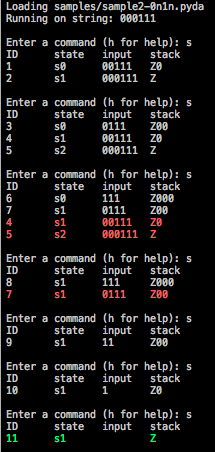
\includegraphics[scale=1.0]{stepping_accept.png}$
\subsubsection{Freeze and Thaw}
Running the same NPDA and string, we can freeze and thaw:\\\\
$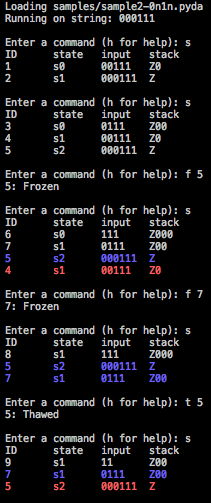
\includegraphics[scale=1.0]{freeze_thaw.png}$


\section{Landon Gilbert-Bland}
I spent most of my time working on the main user interface and interaction with
the program, as well as the ability for freeze and thaw current nodes that were
running.
\subsection{User Interaction}
For the main user interaction with stepping through the states, many aspects were
involved. The first thing we had to do is define exactly what this program should
be able to do, and then provided the user with a very straightforward way of doing it.
We opted to go with a model view controller (MVC) type of approach to separate 
out the parts of this program. The npda.py object acted as the model, and the 
PyDA\_cli.py acted as the view and controller. I decided the best way to do 
this would be to set up an event loop that processed user input, similar to 
a shell, or gdb. After we had defined everything that this program needed to do,
it was a fairly straightforward process to parse the users commands and use it
to modify the underlying state of the program.
\subsection{Freezing and Thawing}
The original problem that we were running into was that it was difficult to process
separate threads, and to know when to spawn new threads, as well as freeze old threads.
What we came up with was instead of creating 'threads' through multiple iterations, we just
used stepper objects (described by Colton bellow), which we didn't reuse. Whenever we
stepped to a new state, instead of continue using the same thread we just created a new
stepper object that had all of the information for that current state. This made it
very simple to freeze current threads from running. All we had to do is move those
objects out of the list that was currently getting processed, and when we thawed a
stepper we move it back into the list that is getting processed. Due to the simple
nature of our implementation this was a very straight forward aspect of the program
to implement.
\subsection{Summary of Work}
I think we did a good job working together to plan out the whole project, then dividing
up the actual coding. Colton coded up the more intensive parts of this program, so
he gets an extra gold star from me.

\begin{itemize}
\item Colton Myers -- $34\%$
\item Andrew Kuhnhausen -- $33\%$
\item Landon Gilbert-Bland -- $33\%$
\end{itemize}

\section{Andrew Kuhnhausen}
I focused on the formal verification, conversion and CLI elements of the
assignment.
\subsection{verify()}
\texttt{verify} ensures that $NPDA=(Q,\Sigma,\Gamma,\delta,q0,Z,F)$ is valid.
The following were asserted in the \texttt{verify()} method:
\begin{itemize}
    \item $\Sigma \ne \{\epsilon\}$
    \item $\epsilon \notin \Sigma$
    \item $q0\in Q$
    \item $F \subseteq Q$
    \item $Z \in \Gamma$
    \item $\{\forall a \in \delta | a \in \Sigma^{*}\}$
    \item $a\in\Sigma\cup\{\epsilon\}$
    \item $A\in\Gamma$
    \item $\alpha\in\Gamma^{*}$
    \item $Q\times(\Sigma\cup\{\epsilon\})\times\Gamma\rightarrow Q\times\Gamma^{*}$
\end{itemize}
\subsection{normalize()}
\texttt{normalize()} is a mapping function from $JSON\rightarrow NPDA$. The
mappings are as follows:
\begin{itemize}
    \item $q0_{JSON}\rightarrow q0_{py}$
    \item $Z_{JSON}\rightarrow Z_{py}$
    \item $\{\forall x\in F_{JSON} \rightarrow F_{py}=\{x_0\cdots x_n\}\}$
    \item $\{\forall x\in Q_{JSON} \rightarrow Q_{py}=\{x_0\cdots x_n\}\}$
    \item $\{\forall x\in\Gamma_{JSON} \rightarrow \Gamma_{py}=\{x_0\cdots x_n\}\}$
    \item $\{\forall x\in\Sigma_{JSON} \rightarrow \Sigma_{py}=\{x_0\cdots x_n\}\}$
    \item $\{\forall (p,a,A,q,\alpha)\in\delta_{JSON},\delta_{a_{JSON}},
                a_{A_{JSON}},
                A_{q_{JSON}},
                q_{\alpha_{JSON}} \rightarrow\\
                \delta_{py}=\{(p,a,A,q,a_0),\cdots,(p,a,A,q,a_n)\}\}$
\end{itemize}

\section{Colton Myers}

My main assignments were PDF output (via Dot), and the main methods which were
to be used to ``step'' our NPDAs.

\subsection{Dot/PDF Output}

The first was fairly straightforward.  On paper, PDAs and NPDAs look
very similar to *FAs which we had done earlier. This meant that I could reuse
much of the code provided to us for printing those automatons to PDFs.  The
one major difference is the way the edges are printed.  This resulted in the
following method which printed the edges from the given NPDA object to the Dot
file:

\begin{minted}{python}
def prEdges(fl, npda):
    print(r'/* The graph itself */', file=fl)
    print(r'""  -> ', dot_san_str(npda["q0"]), ";", file=fl)
    for QcQ in npda["Delta"]:
        print(dot_san_str(QcQ[0]), r' -> ', dot_san_str(QcQ[3]),
              r'[label="', dot_san_str(QcQ[1]) + ',',
              dot_san_str(QcQ[2]) + ';', dot_san_str(QcQ[4]), r'"];', file=fl)
\end{minted}

Note that we used the same notation on the edges as we used in our assignments
and in class, namely \texttt{input, pop; push}.  The only time that the Dot
output is unwieldy is in the case of a CFG to PDA conversion, where there are
many transitions from one state to itself.

The PDF output method, \texttt{pda2pdf()}, just added a few lines to the Dot
output method, \texttt{pda2dot()}, so I will show just the former here:

\begin{minted}{python}
def pda2pdf(npda_obj, pdaname):
    """Generate a .pdf file for the given NPDA object and pdaname

    NOTE:  The .pdf part of the filename should not be included in pdaname
    """
    with open(pdaname + '.dot', 'w') as fl:
        prDotHeader(fl)
        prNodeDefs(fl, npda_obj.pda)
        prOrientation(fl)
        prEdges(fl, npda_obj.pda)
        prClosing(fl)

    os.system("dot -Tps " + pdaname + ".dot > " + pdaname + ".ps")
    os.system("ps2pdf13 " + pdaname + ".ps")
    os.system("rm " + pdaname + ".dot " + pdaname + ".ps")
\end{minted}

\subsection{PDA Stepping Interface}

The PDA stepping interface is the real meat of the PDA.  Basically, we have a
class called a Stepper.  The only things this class stores are an ID, the
remaining input string, the current state, and the current stack.  We have a
different Stepper object for each of the non-deterministic ``forks'' in our PDA,
and we store these Steppers in a list in our NPDA object.  Then, when we want
to progress, or ``step'' our PDA, we call the \texttt{step\_all()} method.
This method goes through each Stepper object in the list, and compares it to
each tuple in the `Delta' of our NPDA, to check for possible continuations.
For each match it finds (matching the input characters, top of the stack, and
current state), it spawns a new Stepper object, containing the state after the
step.  The original Stepper is discarded after all these comparisons, and all
the new Steppers are added to the Stepper list.

The \texttt{step\_all()} method was as follows:

\begin{minted}{python}
def step_all(self):
    """
    Steps though every stepper that we have by 1 step.
    Returns true if there are more states that can be stepped through, and
    false if we cannot do any more stepping (e.g. if the string is not accepted
    by the pda)
    """
    # The new list of valid states after we step every stepper by 1
    new_valid_states = list()
    new_reject_states = list()

    # Step every stepper by 1, and create a list of the new valid states
    for s in self.stepper_list:
        valid_states = s.step(self)
        if not valid_states:
            new_reject_states.append(s)
        new_valid_states.extend(valid_states)

    # Set the new valid states to be the npda.stepper_list
    self.stepper_list = new_valid_states
    # Set the rejected states
    self.reject_list = new_reject_states
\end{minted}

\noindent
\\The \texttt{step()} method was a Stepper method and was as follows:\\

\begin{minted}{python}
def step(self, npda):
    """
    Steps the current Stepper object, returning a list of new Stepper
    objects resulting from any transitions, based on the given npda
    """
    steppers = list()

    for d in npda.pda['Delta']:
        if d[0] == self.state:
            if d[1] == self.inpt[:1] or d[1] == '@':
                # Top of stack is the end of the string, and so we also
                # have to reverse the result using [::-1]
                if d[2] == self.stack[-len(d[2]):][::-1] or d[2] == '@':
                    new_stack = self.stack[:]
                    new_inpt = self.inpt
                    # Pop the specified characters from the stack
                    if not d[2] == '@':
                        new_stack = new_stack[:-len(d[2])]
                    # Push the new characters to the stack
                    if not d[4] == '@':
                        new_stack = new_stack + d[4][::-1]
                    # Consume input character (if not eps (@))
                    if not d[1] == '@':
                        new_inpt = new_inpt[1:]
                    # Create the new Stepper object including new state
                    # and add to the steppers list
                    steppers.append(Stepper(new_inpt, d[3], new_stack))

    # Return finished list of steppers
    return steppers;
\end{minted}

The rest of our program was built on top of these two methods, allowing the
user to either manually control each step or just have the program attempt to
either accept or reject a given string automatically.

\subsection{Summary of Work}

I believe we split up this project very evenly, with everyone chipping in where
needed and pulling their own weight.  Thus, I give the following scores:

\begin{itemize}
\item Colton Myers -- $34\%$
\item Andrew Kuhnhausen -- $33\%$
\item Landon Gilbert-Bland -- $33\%$
\end{itemize}

\end{document}

